%卒論概要テンプレート ver. 3.0

\documentclass[uplatex,twocolumn,dvipdfmx]{jsarticle}
\usepackage[top=22mm,bottom=22mm,left=22mm,right=22mm]{geometry}
\setlength{\columnsep}{10mm}
\usepackage[T1]{fontenc}
\usepackage{txfonts}
\usepackage[expert,deluxe]{otf}
\usepackage[dvipdfmx,hiresbb]{graphicx}
\usepackage[dvipdfmx]{hyperref}
\usepackage{pxjahyper}
\usepackage{secdot}



%以下が本文
%タイトルと学生番号,名前だけ編集すること
\title{\vspace{-5mm}\fontsize{14pt}{0pt}\selectfont 学生生活実態調査のためのデータマイニング手法の提案}
\author{\normalsize プロジェクトマネジメントコース 矢吹研究室 1342045 川手元稀}
\date{}
\pagestyle{empty}
\begin{document}
\fontsize{10.5pt}{\baselineskip}\selectfont
\maketitle





%以下が本文
\section{序論}
千葉工業大学では2001年から学生の意識や考え方を調査するために,毎年「学生生活アンケート」を行っている.
このアンケートの結果は,調査報告書として津田沼校舎や新習志野校舎の図書館等に掲示されている.\cite{a}
アンケートの結果は設問単位で分析されており,設問間の関連は分析されていない.
そこで学生を更に理解するためには設問ごとに分析を行うのではなく,全設問をまとめて分析を行えば理解できるのではないのかと考えた.
そのためにはデータマイニングの手法を利用することが良いと考えた.学生はどのような意識や考えで学校に来ているのか.
データマイニングの手法を利用して「学生生活アンケート」を発展させたいと考えた.

\section{目的}
データマイニングの手法を利用して「学生生活アンケート」を発展させることが目的である.
アンケートの結果は設問単位で分析されており,設問間の関連は分析されていない.
そこで全設問を利用したクラスター分析,対応分析を行ってどのような結果が出るか試す.クラスター分析は学生の行動パターンをグループに分け,群衆の特徴を見つけ出す分析手法である\cite{b}.
対応分析は設問同士の関連性を調べるために使用する.
\section{手法}
本研究は4段階に分かれる.
\begin{enumerate}
\item 千葉工業大学が実施した2015年度版「学生生活アンケート」をGoogleフォームにて作成する.
\item 千葉工業大学の学生100人分のアンケートを集める.
\item 学生の意識や考え方に関するデータに注目し,独自に分析,解析する.
\item 新たな解析法とまとめ方を提案する.
\end{enumerate}
\section{結果}
学生100人分のアンケートデータにクラスター分析を行った結果が図1である.図1の下部にある番号は各学生の番号である.番号同士の位置が近ければ考え方や意識が類似している傾向にある.
\begin{figure}[h]
\centering
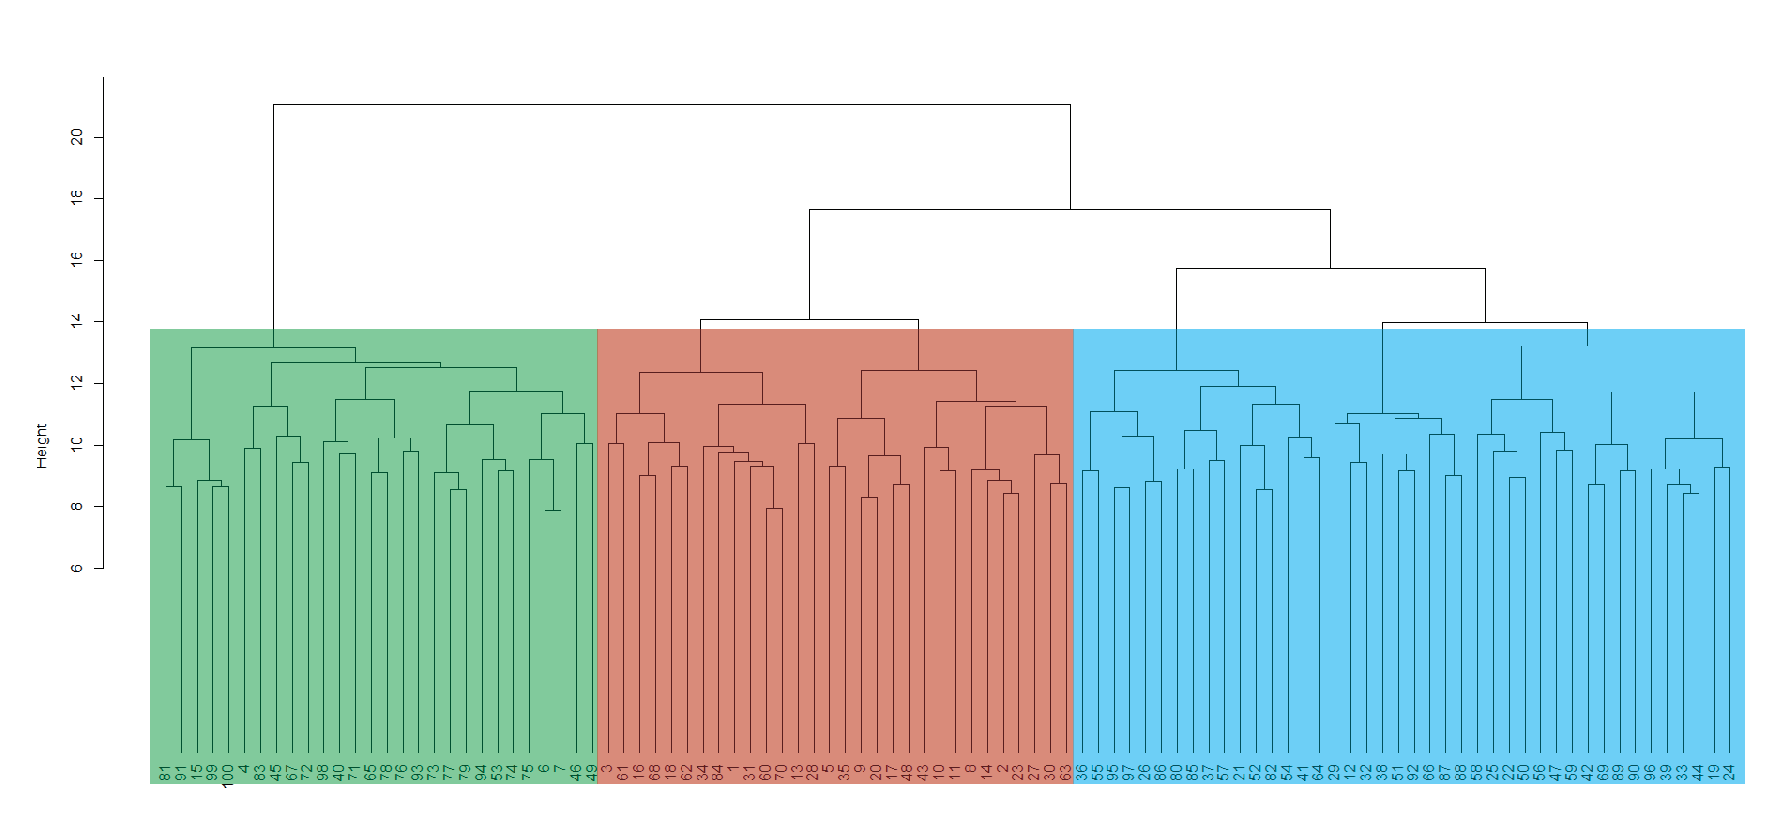
\includegraphics[width=7cm]{clusterresults.pdf}
\caption{学生100人分のクラスター分析}\label{学生100人分のクラスター分析}
\end{figure}
\section{考察}
クラスター分析で考え方や意識が類似している人達をグループにまとめることができる.例えば緑色のグループに属している75,6,7,46,49の5人は,AO入試で入学した人達で進級に若干不安を持っており学生支援センターに行く傾向にあるグループである.このように分けられたグループがどのような考え方や意識を持っている学生なのか理解できる.
\section{結論}
学生の考え方や意識をまとめることができる分析手法を提案した.大学のアンケート結果との相違点は全ての設問を絡めた点である.全ての設問を絡めたことにより人の習性や行動パターンも明らかにした.
\bibliographystyle{junsrt}
\bibliography{biblio}%「biblio.bib」というファイルが必要.
\end{document}
